\documentclass{beamer}
\usepackage{graphicx}

\title{Squirmers: Understanding and Simulation of two interacting squirmers}
\author{Robin and Justine}

\begin{document}
\begin{frame}
    \titlepage
\end{frame}

\begin{frame}{What is a Squirmer ?}
    \begin{columns}[T]
        \begin{column}{0.5\textwidth}
            \begin{itemize}
                \item Introduced by James Lighthill in 1952 \cite{Wikipedia}
                \item Extended by John Blake in 1971 \cite{Wikipedia}
                \item Model for a spherical microswimmer
                \item Cannot model cilia so we impose boundary conditions
                \begin{itemize}
                    \item Tangential speed at the boundary remains constant over time, propelling the squirmers.
                    \item In particullar, we fix the type $\beta$ and the speed $B1$.
                \end{itemize}
            \end{itemize}
        \end{column}
        \begin{column}{0.5\textwidth}
            \centering
            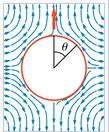
\includegraphics[width=\textwidth]{images/squirmer.png}
            \cite{Wikipedia}
        \end{column}
    \end{columns}
\end{frame}

\begin{frame}{Objectives}
    \begin{itemize}
        \item Understand the "Squirmers" model
        \item Study the dynamics between two squirmers
        \begin{itemize}
            \item Study the interactions between two squirmers
            \item Reformulate the formulas of all present forces and torques (hydrodynamic and collision)
            \item Develop code to calculate the motion of two squirmers
        \end{itemize}
        \item Numerical Experiments
        \begin{itemize}
            \item Verify if our results align with previous studies\cite{Brumley}\cite{Lauga}\cite{Stark}
            \item Verify if changing the value of $\beta$ and the initial distance affect the behavior
        \end{itemize}
    \end{itemize}
\end{frame}

\begin{frame}{Roadmap}
    \begin{center}
        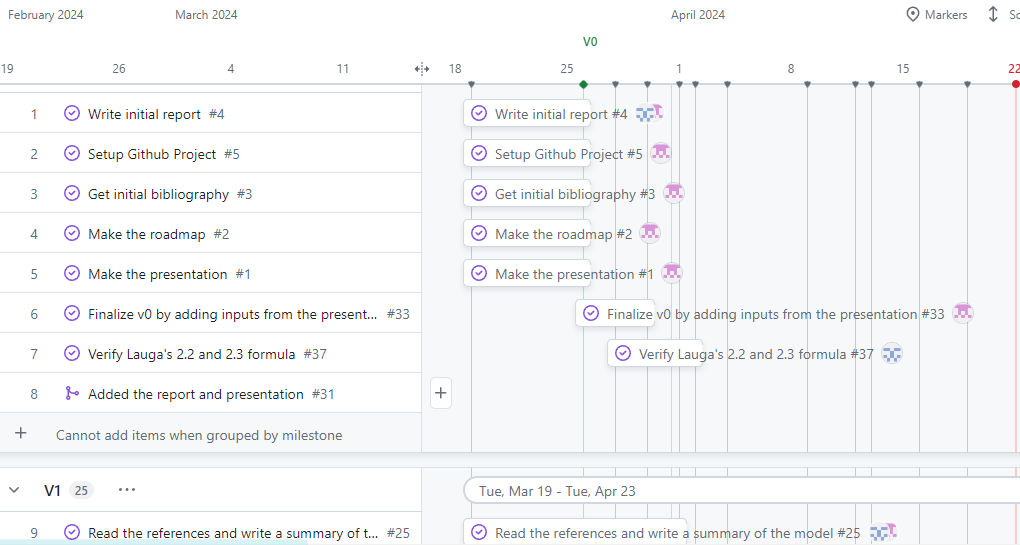
\includegraphics[width=0.9\textwidth]{images/roadmapV0_1.png}
        \vspace{1em} % Ajoute un espace vertical
        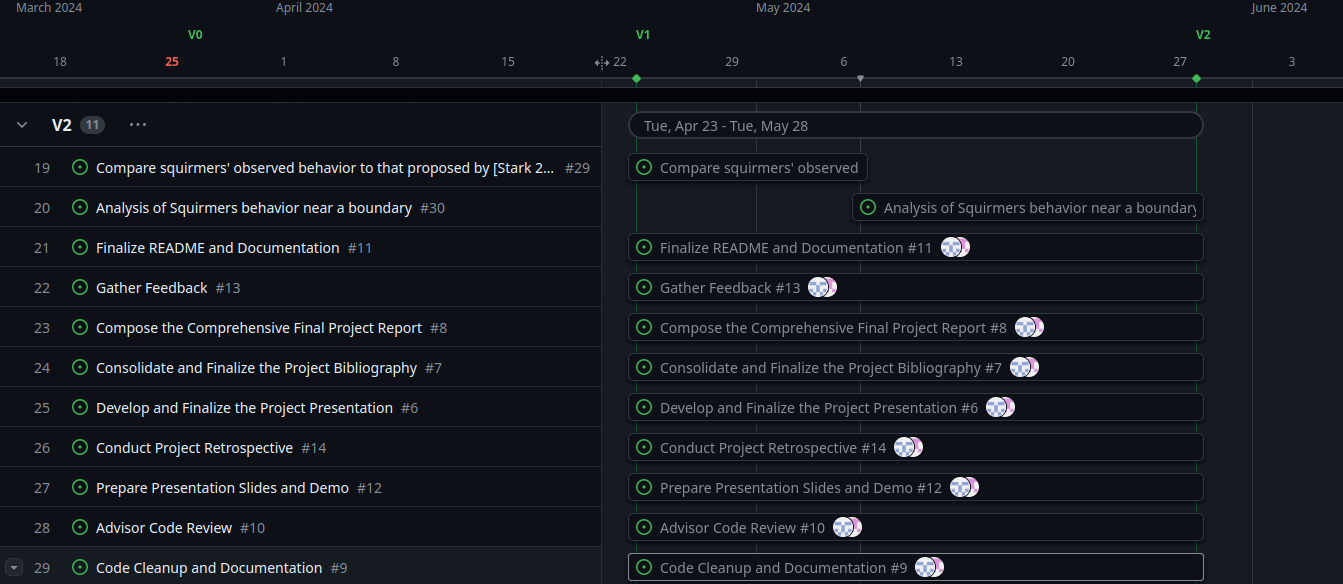
\includegraphics[width=0.9\textwidth]{images/roadmapV0_2.png}
    \end{center}
\end{frame}

\begin{frame}{References}
    \begin{thebibliography}{}
        \bibitem{Brumley} D.R. Brumley and T.J. Pedley, \emph{Stability of arrays of bottom-heavy spherical squirmers}, American Physical Society, 2019
        \bibitem{Lauga} Théry A., Maaß C.C. and Lauga E., \emph{Hydrodynamic interactions between squirmers near walls: far-field dynamics and near-field cluster stability}, Royal Society Open Science, 2023
        \bibitem{Stark} Miloš Knežević,Till Welker \& Holger Stark, \emph{Collective motion of active particles exhibiting non reciprocal orientational interactions}, Scientific Reports, 2022
        \bibitem{Wikipedia} Wikipédia, \emph{Squirmer}, Wikipédia, 2022
    \end{thebibliography}
\end{frame}

\end{document}